\chapter{DASAR TEORI}

Bab ini berisikan dasar teori yang digunakan pada hasil penelitian ini. Beberapa hal yang akan dibahas dalam bab dasar teori ini di antaranya sistem persamaan linear, matriks, fungsi kontinu, dan interpolasi.

\section{Sistem Persamaan Linear}

Bagian ini menjelaskan tentang sistem persamaan linear yang diambil dari buku karya \citep{howard}. Pada bidang dua dimensi, sebuah garis menggunakan sistem koordinat-$xy$ dapat direpresentasikan sebagai persamaan
\begin{equation*}
    ax + by = c,
\end{equation*}
dengan $a$ atau $b$ tidak sama dengan 0. Persamaan ini disebut sebagai persamaan linear dengan dua variabel $x$ dan $y$. Selain pada bidang dua dimensi, sebuah garis juga bisa direpresentasikan sebagai persamaan pada bidang tiga dimensi menggunakan sistem koordinat-$xyz$ berupa
\begin{equation*}
    ax + by + cz = d,
\end{equation*}
dengan $a$, $b$, dan $c$ tidak semuanya 0. Persamaan linear menggunakan sistem koordinat-$xyz$ disebut sebagai persamaan linear dengan tiga variabel $x$,$ y$, dan $z$.
\begin{definisi}
    Jika $a_1, a_2, \dots, a_n$ dan $b$ merupakan bilangan real, maka persamaan
    \begin{equation*}    
    a_1x_1 + a_2x_2 + \dots + a_nx_n =b
    \end{equation*}
    merupakan \textbf{persamaan linear} dengan $n$ variabel $x_1, x_2, \dots, x_n$. Di sini $a_1, a_2, \dots, a_n$ adalah koefisien dari $x_1, x_2, \dots, x_n$ secara berurutan.
\end{definisi} 
\begin{contoh}
    Diberikan persamaan linear
    \begin{align*}
        2x_1 + 3x_2 + x_3 = 1.
    \end{align*}
    Persamaan ini disebut persamaan dengan tiga variabel yaitu $x_1,$ $x_2,$ dan $x_3$.
\end{contoh}
\begin{definisi}
    Kumpulan persamaan linear yang terdiri dari $m$ persamaan linear dengan $n$ variabel $x_1, x_2, \dots, x_n$ ditulis
    \begin{gather*}
        a_{11}x_1 + a_{12}x_2 + \dots + a_{1n}x_n =b_1,\\
        a_{21}x_1 + a_{22}x_2 + \dots + a_{2n}x_n =b_2,\\
        \vdots\\
        a_{m1}x_1 + a_{m2}x_2 + \dots + a_{mn}x_n =b_m,
    \end{gather*}
    disebut sebagai \textbf{sistem persamaan linear} dengan $n$ variabel.
\end{definisi}
\begin{contoh}
    Diberikan sistem persamaan
    \begin{align*}
        2x_1 + 3x_2 = 1,\\
        4x_1 - 2x_2 = 3.
    \end{align*}
    Sistem persamaan ini disebut sistem persamaan dengan dua variabel yaitu $x_1$ dan $x_2$.
\end{contoh}
Di dalam \citep{howard} dijelaskan bahwa sebuah sistem persamaan \mbox{linear} tidak selalu memiliki \mbox{solusi}. Namun, apabila sistem persamaan linear memiliki \mbox{solusi} maka solusi persamaan linear tersebut tunggal atau terdapat tak hingga banyaknya solusi. Sebagai contoh, sistem persamaan linear terdiri dari dua persamaan garis pada bidang dua dimensi dapat dicari solusinya secara geometris dengan mencari titik potong dua garis tersebut. Perpotongan dua garis tersebut tidak selalu ada karena bisa saja kedua garisnya saling sejajar sehingga tidak memiliki titik potong berakibat solusi dari sistem persamaanya tidak ada.

\begin{contoh}
    Diberikan sistem persamaan
    \begin{align*}
        x_1 + 2x_2 = 1. \\
        2x_1 + 4x_2 = 2.
    \end{align*}
    Sistem persamaan tersebut memiliki tak hingga banyaknya solusi.
\end{contoh}

\section{Matriks dan Vektor}
Matriks merupakan rangkaian angka yang membentuk sebuah persegi \mbox{panjang} dengan setiap angka menempati elemen pada baris dan kolom tetentu. Definisi \mbox{dari} matriks, vektor dan operasinya beserta definisi norma diambil dari buku karya \citep{howard}.

\begin{definisi}
Sebuah matriks dinotasikan sebagai
\begin{align*}    
A=
\begin{bmatrix}
a_{11} & a_{12} & \dots & a_{1n}\\
a_{21} & a_{22} & \dots & a_{2n}\\
\vdots & \vdots & \ddots & \vdots\\
a_{m1} & a_{m2} & \dots & a_{mn} 
\end{bmatrix}
\end{align*}
yang disebut sebagai \textbf{matriks berukuran $m \times n$}, dengan $m$ banyak baris dari $A$ dan $n$ banyak kolomnya. 
\end{definisi}

\begin{contoh}
    Diberikan matriks
    \begin{align*}
        B=
\begin{bmatrix}
1 & 2 & -1\\
3 & 0 & -2\\ 
\end{bmatrix}
,C=
\begin{bmatrix}
2 & 5\\
-1 & 3\\ 
\end{bmatrix}.
    \end{align*}
    Matriks $B$ merupakan matriks $2 \times 3$ sedangkan matriks $C$ merupakan matriks $2 \times 2$.
\end{contoh}
Sebuah matriks merupakan matriks persegi jika $m=n$, yaitu matriks \mbox{tersebut} memiliki jumlah barisnya yang sama dengan jumlah kolomnya. Selain memiliki bentuk persegi panjang sebuah matriks juga memiliki ciri penamaan sendiri, yaitu sebuah matriks biasanya dinotasikan menggunakan huruf besar. 

Setiap elemen matriks diidentifikasi berdasarkan baris dan kolom tempat elemen tersebut berada. Baris dihitung dari atas ke bawah sedangkan kolom \mbox{dihitung} dari kiri ke kanan. Sebagai contoh, elemen matriks $B$ yang berada pada baris ke-2 dan kolom pertama adalah 3.

Matriks yang hanya memiliki satu baris atau satu kolom saja disebut \mbox{sebagai} vektor. Sebuah vektor kolom adalah matriks yang berukuran $m \times 1$ sedangkan \mbox{vektor} baris merupakan matriks yang berukuran $1 \times n$. Berbeda dengan matriks, sebuah vektor biasanya dinotasikan menggunakan hurup kecil. 
\begin{definisi}
\textbf{Vektor kolom} dan \textbf{vektor baris} dinotasikan sebagai
\begin{align*}
    u=\begin{bmatrix}
        a_1\\
        a_2\\
        \vdots\\
        a_m
    \end{bmatrix},
    v=\begin{bmatrix}
        a_1 & a_2 & \dots & a_n
    \end{bmatrix}.
\end{align*}
Vektor $u$ merupakan vektor kolom berukuran $m \times 1$ dan vektor $v$ merupakan vektor baris berukuran $1 \times n$.
\end{definisi}

\begin{contoh}    
Diberikan vektor
\begin{align*}    
u=
\begin{bmatrix}
-2 \\
3 \\
4 \\ 
\end{bmatrix} 
v=
\begin{bmatrix}
    1 & 4 & -1 & -2
\end{bmatrix}.
\end{align*}
Vektor $u$ adalah vektor kolom yang berukuran $3 \times 1$ dan vektor $v$ adalah vektor baris yang berukuran $1 \times 4$.
\end{contoh}

Sebuah sistem persamaan linear yang terdiri dari $m$ persamaan linear \mbox{dengan} $n$ buah variabel dapat direpresentasikan oleh sebuah persamaan matriks $Ax=b$, dengan $A$ matriks kofisien berukuran $m \times n$ serta $x$ dan $b$ vektor berukuran $n \times 1$.

\begin{definisi}
    Diberikan sistem persamaan linear dengan $n$ varibel
    \begin{gather*}
        a_{11}x_1 + a_{12}x_2 + \dots + a_{1n}x_n =b_1,\\
        a_{21}x_1 + a_{22}x_2 + \dots + a_{2n}x_n =b_2,\\
        \vdots\\
        a_{m1}x_1 + a_{m2}x_2 + \dots + a_{mn}x_n =b_m.
    \end{gather*}
    Sistem persamaan linear di atas dapat dinyatakan dalam \textbf{persamaan matriks $Ax=b$}, dengan
    \begin{align*}
        A=
        \begin{bmatrix}
a_{11} & a_{12} & \dots & a_{1n}\\
a_{21} & a_{22} & \dots & a_{2n}\\
\vdots & \vdots & \ddots & \vdots\\
a_{m1} & a_{m2} & \dots & a_{mn}
\end{bmatrix},
x=\begin{bmatrix}
    x_1\\
    x_2\\
    \vdots\\
    x_n
\end{bmatrix},
b=\begin{bmatrix}
    b_1\\
    b_2\\
    \vdots\\
    b_m
\end{bmatrix}.
    \end{align*}
\end{definisi}
\begin{contoh}
    Diberikan sistem persamaan linear
    \begin{align*}
        a + 2b - 3c = 6,\\
        2a - 3b + 5c = 2,\\
        -a + 4b - 1c = -3.
    \end{align*}
    Sistem persamaan tersebut dapat dituliskan sebagai persamaan matriks berikut
    \begin{align*}
        \begin{bmatrix}
            1&2&-3\\
            2&-3&5\\
            -1&4&-1
        \end{bmatrix}
        \begin{bmatrix}
            a\\
            b\\
            c
        \end{bmatrix}
        =
        \begin{bmatrix}
            6\\
            2\\
            -3
        \end{bmatrix}.
    \end{align*}
\end{contoh}
\subsection{Operasi Matriks dan Vektor}

Matriks memiliki operasi aljabar antar matriks yang dapat menghasilkan sebuah \mbox{matriks} baru. Operasi aljabar pada matriks di antaranya adalah operasi \mbox{penjumlahan}, pengurangan, dan perkalian. Sebelum mendefinisikan operasi tersebut didefinisikan terlebih dahulu tentang kesamaan matriks.

\subsubsection{Kesamaan Matriks}

Kesamaan matriks didefinisikan untuk dua buah matriks yang sama besar. Dalam hal ini, jika dua buah matriks sama, maka operasi yang dilakukan pada kedua matriks tersebut memiliki hasil yang sama. Berikut definisi kesamaan matriks.

\begin{definisi}
Dua buah matriks dikatakan \textbf{sama} jika dan hanya jika kedua \mbox{matriks} tersebut memiliki ukuran yang sama dan semua elemen yang bersesuaian juga \mbox{sama}.
\end{definisi}

\begin{contoh}
Diberikan matriks $A$ dan $B$ sebagai
\begin{align*}    
A=
\begin{bmatrix}
2 & 3 & 1 & 0\\
1 & 1 & -4 & 0\\
-1 & 2 & -2 & 3\\
7 & 4 & 1 & -2\\ 
\end{bmatrix}
,B=
\begin{bmatrix}
2 & 3 & 1 & 0\\
1 & 1 & -4 & 0\\
-1 & 2 & -2 & 3\\
7 & 4 & 1 & -2\\ 
\end{bmatrix}.
\end{align*}
Matriks $A$ dan $B$ pada contoh merupakan matriks yang sama karena $A$ dan $B$ memiliki ukuran yang sama yaitu $4 \times 4$ dan semua elemennya yang bersesuaian sama.
\end{contoh}

\subsubsection{Penjumlahan Matriks}
\begin{definisi}
    Jika $A$ dan $B$ matriks dengan ukuran yang sama, maka \textbf{jumlahan $A+B$} merupakan matriks yang diperoleh dengan menjumlahkan setiap elemen matriks $A$ dan $B$ yang bersesuaian.
\end{definisi}
\begin{contoh}
Diberikan matriks $A$ dan $B$ sebagai
\begin{gather*} 
        A=
        \begin{bmatrix}
        3 & 1 & 2 & 1\\
        2 & 3 & -2 & 1\\
        -1 & 2 & 0 & 2\\
        \end{bmatrix}
        ,B=
        \begin{bmatrix}
        2 & 1 & 4 & 3\\
        2 & 7 & -5 & 2\\
        -3 & 1 & -2 & 2\\
        \end{bmatrix}, \\
        A+B=
        \begin{bmatrix}
        5 & 2 & 6 & 4\\
        4 & 10 & -7 & 3\\
        -4 & 3 & -2 & 4\\
        \end{bmatrix}.
\end{gather*}
Matriks $A+B$ merupakan matriks yang diperoleh dengan menjumlahkan elemen-elemen yang bersesuaian pada matriks $A$ dan $B$.
\end{contoh}

Seperti operasi penjumlahan pada bilangan real, operasi penjumlahan pada matriks bersifat komutatif dan asosiatif sehingga apabila diberikan matriks $A$, $B$, dan $C$ yang berukuran sama, maka berlaku
\begin{gather*}
    A+B = B+A, \\
    A+(B+C) = (A+B)+C.
\end{gather*}
\begin{contoh}\label{A+B Contoh}
Diberikan matriks $A$, $B$, dan $C$ sebagai
\begin{gather*} 
        A=
        \begin{bmatrix}
        3 & 1 & 2 & 1\\
        2 & 3 & -2 & 1\\
        -1 & 2 & 0 & 2\\
        \end{bmatrix}
        ,B=
        \begin{bmatrix}
        2 & 1 & 4 & 3\\
        2 & 7 & -5 & 2\\
        -3 & 1 & -2 & 2\\
        \end{bmatrix} 
        ,C=
        \begin{bmatrix}
        1 & 1 & 2 & 1\\
        2 & 4 & 0 & 2\\
        -1 & 0 & -1 & 4\\
        \end{bmatrix}.
        \end{gather*}
        Dengan menjumlahkan matriks $A$ dan $B$ diperoleh
        \begin{gather*}
        A+B=B+A=
        \begin{bmatrix}
        5 & 2 & 6 & 4\\
        4 & 10 & -7 & 3\\
        -4 & 3 & -2 & 4\\
        \end{bmatrix}.
        \end{gather*}
        Dengan menjumlahkan matriks $A$, $B$, dan $C$ diperoleh
        \begin{gather*}  
        A+(B+C) = (A+B)+C=
        \begin{bmatrix}
        6 & 3 & 9 & 5\\
        6 & 14 & -7 & 5\\
        -5 & 3 & -3 & 8\\
        \end{bmatrix}. \\
\end{gather*}
\end{contoh}
Untuk operasi pengurangan pada matriks $A$ dan $B$ yang berukuran sama, $A-B$ adalah matriks yang diperoleh dengan mengurangkan elemen pada matriks $A$ dengan elemen pada matriks $B$ yang bersesuaian. Sebagai contoh, diambil matriks $A$ dan $B$ pada Contoh \ref{A+B Contoh} sehingga diperoleh hasil pengurangan matriksnya berupa matriks
\begin{gather*}
    A-B=
    \begin{bmatrix}
        1 & 0 & -2 & -2\\
        0 & -4 & 3 & -1\\
        2 & 1 & 2 & 0\\
    \end{bmatrix}.
\end{gather*}


\subsubsection{Perkalian Matriks dengan Skalar}
\begin{definisi}
    Jika A sebarang matriks dan k sebarang bilangan real, maka\textbf{ perkalian skalar kA} adalah matriks yang diperoleh dengan mengalikan setiap elemen A dengan k.
\end{definisi}
\begin{contoh}
Diberikan matriks $A$ dan skalar $k$ berikut
\begin{gather*} 
        A=
        \begin{bmatrix}
        3 & 1 & 2 & 1\\
        2 & 3 & -2 & 1\\
        -1 & 2 & 0 & 2\\
        \end{bmatrix}
        ,k=2.
        \end{gather*}
        Diperoleh
        \begin{gather*}
        kA=2\begin{bmatrix}
        3 & 1 & 2 & 1\\
        2 & 3 & -2 & 1\\
        -1 & 2 & 0 & 2\\
        \end{bmatrix}=
        \begin{bmatrix}
        2(3) & 2(1) & 2(2) & 2(1)\\
        2(2) & 2(3) & 2(-2) & 2(1)\\
        2(-1) & 2(2) & 2(0) & 2(2)\\
        \end{bmatrix}=
        \begin{bmatrix}
        6 & 2 & 4 & 2\\
        4 & 6 & -4 & 2\\
        -2 & 4 & 0 & 4\\
        \end{bmatrix}.
\end{gather*}

\end{contoh}

\subsubsection{Perkalian Matriks dan Vektor}
Operasi perkalian matriks dan vektor merupakan operasi yang sangat penting dalam menyelasaikan sebuah persamaan matriks. Perkalian matriks dan perkalian vektor melibatkan hasil kali elemen-elemen yang ada dalam matriks dan vektor tersebut.
\begin{definisi}
    Diberikan vektor $u=\begin{bmatrix}
            u_1&u_2&\dots&u_n
        \end{bmatrix}$ dan vektor $v=\begin{bmatrix}
            v_1\\
            v_2\\
            \vdots\\
            v_n
        \end{bmatrix}$. Hasil \textbf{perkalian vektor} u dan v, dinotasikan dengan uv, didefinisikan sebagai
    \begin{align*}
        uv=u_1v_1 + u_2v_2 + \dots + u_nv_n.
    \end{align*}
\end{definisi}
\begin{contoh}
Diberikan vektor $u$ dan $v$ berikut
\begin{align*}
    u=\begin{bmatrix}
            3&-2&1
        \end{bmatrix},
        v=\begin{bmatrix}
            1\\
            3\\
            2
        \end{bmatrix}.
\end{align*}
Diperoleh hasil kali vektor $uv$ adalah
\begin{align*}
    uv=(3)(1) + (-2)(3) + (1)(2)=-1.
\end{align*}
\end{contoh}
Setelah didefinisikan operasi perkalian pada vektor, akan didefinisikan operasi perkalian antar matriks. Operasi perkalian pada matriks melibatkan vektor-vektor baris dan kolom pada matriks sehingga diperoleh matriks baru dari perkalian vektor baris dan kolom tersebut. Dalam mengalikan dua buah matriks $A$ dan $B$ menghasilkan matriks $AB$, matriks $A$ harus memiliki jumlah kolom yang sama dengan jumlah baris matriks $B$.
\begin{definisi}
    Diberikan matriks $$A=\begin{bmatrix}
a_{11} & a_{12} & \dots & a_{1n}\\
a_{21} & a_{22} & \dots & a_{2n}\\
\vdots & \vdots & \ddots & \vdots\\
a_{m1} & a_{m2} & \dots & a_{mn}
\end{bmatrix},$$ dan matriks $$B=\begin{bmatrix}
b_{11} & b_{12} & \dots & b_{1p}\\
b_{21} & b_{22} & \dots & b_{2p}\\
\vdots & \vdots & \ddots & \vdots\\
b_{n1} & b_{n2} & \dots & b_{np}
\end{bmatrix}$$ dengan $m,n,p \in \N$.
 Hasil \textbf{perkalian matriks} A dan B, dinotasikan dengan AB, didefinisikan sebagai
\begin{align*}
AB=\begin{bmatrix}
c_{11} & c_{12} & \dots & c_{1p}\\
c_{21} & c_{22} & \dots & c_{2p}\\
\vdots & \vdots & \ddots & \vdots\\
c_{m1} & c_{m2} & \dots & c_{mp}
\end{bmatrix},
    \end{align*}
    dengan $c_{ij}$ elemen pada baris ke-$i$ dan kolom ke-$j$ dari matriks $AB$
    \begin{align*}
        c_{ij}=a_{i1}b_{1j}+a_{i2}b_{2j}+a_{i3}b_{3j}+\dots+a_{in}b_{nj}.
    \end{align*}
\end{definisi}
\begin{contoh}
Diberikan matriks $A$ dan $B$ sebagai berikut
    \begin{gather*}
        A=
        \begin{bmatrix}
            1 & -1 & 3 & 2\\
            1 & 1 & -4 & 2\\
            2 & 4 & 2 & 1
        \end{bmatrix},
        B=
        \begin{bmatrix}
            3 & 3 & 1\\
            -3 & 1 & 2\\
            1 & 7 & -3\\
            -6 & 1 & 2
        \end{bmatrix}.
    \end{gather*}
    Diperoleh hasil kali matriks $AB$ adalah
    \begin{gather*}
        AB=
        \begin{bmatrix}
            -3 & 25 & -6\\
            -16 & -22 & 19\\
            -10 & 25 & 6
        \end{bmatrix}.
    \end{gather*}
\end{contoh}

\begin{definisi}
    Misal $\textbf{A}=
    \begin{bmatrix}
    a_1 & a_2 & \dots & a_n \\    
    \end{bmatrix}$
    merupakan matriks $m \times n$, dengan $a_1$, $a_2$, \dots, $a_n$ adalah kolom-kolom dari $\textbf{A}$. Jika $x=
    \begin{bmatrix}
    x_1 \\
    x_2 \\
    \vdots \\
    x_n
    \end{bmatrix}$ adalah vektor kolom berukuran $n \times 1$, Ax didefinisikan sebagai vektor kolom hasil \textbf{perkalian matriks dan vektor} berukuran $m \times 1$ berikut:
    \begin{equation*}
        Ax = x_1a_1 + x_2a_2 + \dots + x_na_n
    \end{equation*}
\end{definisi}
\begin{contoh}
Diberikan matriks $A$ dan vektor $x$ sebagai berikut
\begin{gather*}
     A=
    \begin{bmatrix}
    3 & 1 & 2 & 1\\
    2 & 3 & -2 & 1\\
    -1 & 2 & 0 & 2\\
    \end{bmatrix},
    x=
    \begin{bmatrix}
    1 \\
    2 \\
    1 \\
    0
    \end{bmatrix}.
\end{gather*}
Diperoleh $Ax$ berupa
\begin{gather*}
    Ax = 
    1\begin{bmatrix}
    3 \\
    2 \\
    -1\\
    \end{bmatrix}+
    2\begin{bmatrix}
    1 \\
    3 \\
    2 \\
    \end{bmatrix}+
    1\begin{bmatrix}
    2 \\
    -2 \\
    0 \\
    \end{bmatrix}+
    0\begin{bmatrix}
    1\\
    1\\
    2\\
    \end{bmatrix} =
    \begin{bmatrix}
    7\\
    6\\
    3\\
    \end{bmatrix}.
\end{gather*}
\end{contoh}

\subsection{Norma}
Operasi pada sebuah matriks ataupun vektor tidak selalu memiliki output matriks atau vektor tetapi juga bisa memiliki output bernilai bilangan real. Salah satu operasi pada vektor yang tidak menghasilkan matriks atau vektor adalah norma.

\begin{definisi}\citep{olver}
    Sebuah \textbf{norma} dalam ruang vektor $V$ adalah fungsi yang memetakan vektor $v \in V$ ke bilangan real nonnegatif. Norma dari $v \in V$ dinotasikan $||v||$, sehingga untuk setiap $v, w \in V$ dan $c \in \R$ memenuhi aksioma berikut:
    \begin{enumerate}
        \item $||v|| \geq 0$, dengan $||v|| = 0$ jika dan hanya jika $v=0$,
        \item $||cv|| = |c|||v||$,
        \item $||v+w|| \leq ||v|| + ||v||$.
    \end{enumerate}
\end{definisi}

Salah satu norma di dalam ruang vektor $\R^n$ adalah norma maksimum yang didefinisikan sebagai
$$||v||_\infty = \max(|v_1|,|v_2|,\dots,|v_n|),$$
untuk setiap $v \in R^n$. Norma maksimum dibutuhkan dalam penelitian ini untuk membuktikan beberapa teorema di dalam hasil penelitian.
\begin{contoh}
Diberikan vektor $v$ sebagai berikut
    \begin{align*}
        v=
        \begin{bmatrix}
            2\\
            1\\
            -3\\
            2
        \end{bmatrix}.
    \end{align*}
    Vektor $v$ merupakan sebuah vektor kolom berukuran $4 \times 1$ yang nilai norma maksimumnya adalah
    \begin{equation*}
        ||v||_\infty=\max(|2|,|1|,|-3|,|2|)=\max(2,1,3,2)=3.
    \end{equation*}
\end{contoh}

\section{Fungsi Kontinu}
Pada bagian ini akan dijabarkan definisi fungsi yang kontinu yang diambil dari \citep{bartle} yang menjelaskan secara detail terkait fungsi kontinu.
\begin{definisi}
    Misal $A \subseteq \R$, $f:A\to\R$, dan $c \in A$. Fungsi f dikatakan \textbf{kontinu di titik $c$} jika untuk setiap $\epsilon > 0$, terdapat $\delta > 0$ sehingga untuk setiap $x \in A$ yang memenuhi $|x-c| < \delta$, maka berlaku $|f(x) - f(c)| < \epsilon$.
\end{definisi}
\begin{contoh}
    Diberikan fungsi $f:\R \to \R$ yang didefinisikan sebagai $f(x)=x^2+2x-3$ untuk setiap $x\in\R$. Fungsi $f$ kontinu dititik $c=1$ karena untuk setiap $\epsilon>0$, terdapat $\delta=\min(\epsilon/4,1/2)>0$ sehingga untuk setiap $|x-1|<\delta$ berlaku
    \begin{align*}
        |x^2+2x-3|=&|(x-1)(x-1-2)|\\
        \leq&|x-1|(|x-1|+2)\\
        <&\frac{\epsilon}{4}(\frac{1}{2}+2)<\frac{3\epsilon}{4}<\epsilon.
    \end{align*}
\end{contoh}
Setelah didefinisikan mengenai kekontinuan fungsi pada suatu titik, selanjutnya akan didefinisikan mengenai fungsi yang kontinu.
\begin{definisi}
Sebuah fungsi $f:A\to\R$ dikatakan \textbf{kontinu} jika $f$ kontinu di setiap titik $x\in A$.
\end{definisi}
\begin{contoh}
    Fungsi $f:\R\to\R$ dengan $f(x)=x$ untuk setiap $x\in\R$ merupakan fungsi kontinu karena untuk setiap $x_0\in\R$ dan untuk setiap $\epsilon>0$, terdapat \mbox{$\delta=\epsilon>0$} sehingga untuk setiap $|x-x_0|<\delta$ berlaku $$|f(x)-f(x_0)|=|x-x_0|<\delta=\epsilon.$$
\end{contoh}
\section{Turunan}
Pada bagian ini akan dijelaskan mengenai konsep-konsep dasar terkait turunan. Jika fungsi $f$ memiliki turunan pada titik $c$, maka nilai turunannya pada titik $c$ dinotasikan sebagai $f'(c)$
\begin{definisi}
    Misal $I \subseteq \R$ merupakan interval, $f:I \to \R$, dan $c \in I$. \textbf{Turunan} dari $f$ di titik $c$ dituliskan sebagai $f'(c)$ didefinisikan sebagai
    \begin{align*}
        f'(c)=\lim_{x \to c}\frac{f(x)-f(c)}{x-c}.
    \end{align*}
    Untuk kasus ketika $c$ merupakan titik ujung dari interval $I$, maka turunan di titik $c$ didefinisikan sebagai limit dari satu sisinya saja.
\end{definisi}
\newpage
\begin{contoh}
    Diberikan fungsi $f:\R\to\R$ dengan $f(x)=x^2+3x-2$ untuk setiap $x\in\R$. Nilai turunan fungsi $f$ di titik 2 adalah
    \begin{align*}
        f'(2)=&\lim_{x\to2}\frac{f(x)-f(2)}{x-2}\\
        =&\lim_{x\to2}\frac{(x^2+3x-2)-8}{x-2}\\
        =&\lim_{x\to2}\frac{x^2+3x-10}{x-2}\\
        =&\lim_{x\to2}\frac{(x-2)(x+5)}{x-2}\\
        =&\lim_{x\to2}(x+5)=7.
    \end{align*}
\end{contoh}
Dalam hal $f$ merupakan fungsi yang punya turunan pada setiap titik di domainnya diperoleh $f'$ juga merupakan fungsi. Jika fungsi $f'$ juga mempunyai turunan pada domainnya, maka kita bisa mendefinisikan fungsi baru $f''=(f')'$ yang disebut sebagai turunan kedua dari $f$. Apabila hal ini dilanjutkan hingga $n$ kali maka diperoleh $f^{(n)}$ yang disebut sebagai turunan ke-$n$ dari fungsi $f$. 

\begin{definisi}
Misal $I \subseteq \R$ merupakan interval dan fungsi $f:I \to \R$. Fungsi $f$ dikatakan sebagai fungsi yang mulus jika fungsi $f$ memiliki turunan fungsi yang kontinu pada interval $I$.
\end{definisi}
\begin{contoh}
    Diberikan fungsi $f:[1,2] \to\R$ dengan $f(x)=x^2+3x-2$, untuk setiap $x\in [1,2]$. Fungsi $f$ memiliki turunan $f'(x) = 2x + 3$,  untuk setiap $x\in [1,2]$. Karena $f'$ kontinu pada interval $[1,2]$, maka fungsi $f$ adalah fungsi yang mulus.
\end{contoh}

Setelah didefinisikan fungsi mulus, akan didefinisikan tentang regularitas fungsi.

\begin{definisi}
    Misal fungsi $f:[a,b] \to \R$. Fungsi $f$ dikatakan memiliki regularitas $C^n$ pada interval $[a,b]$ jika fungsi $f$ dapat diturunkan sebanyak $n$ kali dan $f^{(n)}$ kontinu pada interval $[a,b]$. Lebih lanjut himpunan fungsi dengan regularitas $C^n$ pada interval $[a,b]$ dinotasikan $C^n[a,b]$.
\end{definisi}
\begin{contoh}
    Diberikan fungsi $f:[1,3] \to \R$, dengan 
    $$f(x) = 
    \begin{cases}
        1 + x &, x \in [1,2],\\
        -2 x^3 + 15 x^2 - 35 x + 29 &, x\in [2,3]. 
    \end{cases}$$ Diperoleh 
    $$f'(x) =  
    \begin{cases}
        1 &, x \in [1,2],\\
        -6 x^2 + 30 x - 35 &, x\in [2,3],
    \end{cases}$$ 
    sehingga $f'$ kontinu pada interval $[1,3]$. Dapat disimpulkan fungsi $f \in C^1[1,3]$.
\end{contoh}

Selanjutnya, akan dibahas mengenai turunan fungsi pada maksimum lokal dan minimum lokal fungsi tersebut.
\begin{definisi}
    Misal $f:I \to \R$, I sebuah interval. Nilai fungsi $f$ di titik $c$ adalah \textbf{maksimum lokal} (minimum lokal) dari $f$ jika terdapat $\delta>0$ sehingga 
    $$f(x) \leq f(c) (f(x) \geq f(c)),$$
    untuk setiap $x \in I \cap (c-\delta,c+\delta)$. Lebih lanjut $f(c)$ adalah maksimum global (minimum global) dari $f$ jika $f(x) \leq f(c) (f(x) \geq f(c))$, untuk setiap $x \in I$.
\end{definisi}
\begin{contoh}
    Diberikan fungsi $f:[1,5] \to \R$ dengan $f(x)=-x^2+6x-8$ untuk setiap \mbox{$x \in [1,5]$}.  $f(3)=1$ adalah maksimum lokal dari $f$ karena terdapat $\delta = 1$ sehingga $-x^2+6x-8 \leq 1$ untuk setiap $x \in [1,5] \cap (2,4)$.
\end{contoh}

Definisi dari maksimum lokal di sini diambil dari \citep{thomas} sebagai nilai fungsi yang terbesar jika dibandingkan dengan nilai fungsi pada titik di sekitarnya. Selain itu, apabila sebuah maksimum lokal ternyata memiliki nilai fungsi terbesar pada domain fungsinya, maka maksimum lokal tersebut merupakan maksimum global. Hal yang sama juga berlaku pada minimum lokal.

Berikutnya diberikan teorema yang berkaitan dengan maksimum lokal dan minimum lokal yang diambil dari \citep{thomas}.
\begin{teorema}\label{2.4.5}
    Misal $f:[a,b] \to \R$ dan misal $f$ punya maksimum lokal atau minimum lokal di titik $c \in (a,b)$. Jika $f$ memiliki turunan pada $c$ maka $f'(c)=0$.
\end{teorema}
\begin{proof}
    Tanpa mengurangi keumuman, dimisalkan $f$ memiliki maksimum lokal di $c\in(a,b)$ dan dapat diturunkan di titik tersebut. Diasumsikan $f'(c) = L_1 > 0$, sehingga $\lim_{x \to c} \frac{f(x) - f(c)}{x-c} = L_1 > 0$. Dipilih $\epsilon = \frac{L_1}{2} > 0$. Terdapat $\delta_1 > 0$, sehingga untuk setiap  $x \in [a,b]$ dan $0 < |x - c| < \delta_1$ berlaku,
    \begin{align*}
        \left|\frac{f(x) - f(c)}{x-c} - L_1\right| < \frac{L_1}{2}.
    \end{align*}
    Diperoleh
    \begin{align*}
        \frac{f(x) - f(c)}{x-c} > \frac{L_1}{2} > 0,
    \end{align*}
    untuk setiap $x \in [a,b]$ dan $0 < |x - c| < \delta_1$.
    Jika $x-c > 0$, maka $f(x) > f(c)$ dan jika $x-c < 0$, maka $f(x) < f(c)$. Hal ini menyebabkan kontradiksi, yaitu $f(c)$ bukan maksimum lokal. Dapat disimpulkan bahwa tidak mungkin $f'(c) > 0$.

    Dengan cara yang sama diasumsikan $f'(c) = L_2 < 0$, sehingga $\lim_{x \to c} \frac{f(x) - f(c)}{x-c} = L_2 < 0$. Dipilih $\epsilon = -\frac{L_2}{2}$. Terdapat $\delta_2 > 0$, sehingga untuk setiap $x \in [a,b]$ dan $0 < |x - c| < \delta_2$ berlaku,
    \begin{align*}
        \left|\frac{f(x) - f(c)}{x-c} - L_2\right| < -\frac{L_2}{2}.
    \end{align*}
    Diperoleh
    \begin{align*}
        \frac{f(x) - f(c)}{x-c} < \frac{L_2}{2} < 0,
    \end{align*}
    untuk setiap $x \in [a,b]$ dan $0 < |x - c| < \delta_2$.
    Jika $x-c > 0$, maka $f(x) < f(c)$ dan jika $x-c < 0$, maka $f(x) > f(c)$. Hal ini menyebabkan kontradiksi, yaitu $f(c)$ bukan maksimum lokal. Dapat disimpulkan bahwa tidak mungkin $f'(c) < 0$.
    
    Dari kedua asumsi terjadi kontradiksi bahwa $f(c)$ bukan maksimum lokal sehigga dapat disimpulkan $f'(c) = 0$.
    % Diperoleh terdapat $\delta_0 > 0$ sehingga  $f(x) \leq f(c)$, untuk setiap \mbox{$x \in I \cap (c-\delta_0,c+\delta_0)$}. Didefinisikan
    % \begin{align*}
    %     y^\star:=\min_{x\in I \cap (c-\delta_0,c+\delta_0)}f(x).
    % \end{align*}
    % Diambil sebarang $\epsilon > 0$. Dipilih $\delta = \min(\delta_0/2, \epsilon/|y^{\star}-f(c)|)$. Diperoleh bahwa untuk setiap $x \in I$ dengan $|x-c|<\delta$ berlaku
    % \begin{align*}
    %     \left|\frac{f(x)-f(c)}{x-c}\right|=\frac{|f(x)-f(c)|}{|x-c|}<\frac{|f(x)-f(c)|}{|y^\star-f(c)|}\epsilon < \epsilon.
    % \end{align*}
    % Jadi dapat disimpulkan $f'(c)=0$.
\end{proof}

Setelah didefinisikan teorema terkait maksimum lokal, akan diberikan teorema yang dibutuhkan dalam beberapa pembuktian berikutnya.

\begin{teorema}\label{ifconvthenbound}
Jika barisan $(x_n)$ adalah barisan pada bilangan real yang konvergen, maka barisan $(x_n)$ terbatas.
\end{teorema}

\begin{proof}
    Dimisalkan $(x_n)$ adalah barisan pada bilangan real yang konvergen  sehingga $lim(x_n) = x$, untuk suatu $x \in \R$. Jika diambil sebarang $\epsilon > 0$, maka terdapat bilangan bulat $K$ dengan $|x_n - x| < \epsilon$, untuk setiap $n \geq K$. Diperoleh
    \begin{align*}
        |x_n| = |x_n - x + x| \leq |x_n - x| + |x| < \epsilon + |x|.
    \end{align*}
    Jika diambil
    \begin{align*}
        M = \sup\{|x_1|,|x_2|,\dots,|x_{K-1}|, \epsilon +|x|\},
    \end{align*}
    maka $|x_n| \leq M$, untuk setiap $n \in \N$.
\end{proof}

Dari Teorema \ref{ifconvthenbound} disimpulkan bahwa setiap barisan yang konvergen merupakan barisan yang terbatas.

\begin{teorema}\label{ifmonotonterbatasthenvonf}
    Sebuah barisan bilangan real yang monoton bersifat konvergen jika dan hanya jika barisannya terbatas. 
\end{teorema}

\begin{proof}
    Berdasarkan Teorema \ref{ifconvthenbound} dapat disimpulkan bahwa sebuah barisan konvergen pasti terbatas. Selanjutnya, akan dibuktikan bahwa barisan monoton terbatas merupakan barisan konvergen.

    Tanpa mengurangi keumuman diambil sebarang barisan monoton naik dan terbatas $X = (x_n)$. Dikarenakan $X$ terbatas, maka terdapat bilangan real $M$ sehingga $x_n \leq M$, untuk setiap $n \in \N$. Dikarenakan sifat kelengkapan himpunan bilangan real yaitu setiap himpunan bilangan real tak kosong yang terbatas ke atas pasti memiliki nilai supremum, maka terdapat bilangan real $x^\star = \sup\{x_n : n \in \N\}$.

    Diambil sebarang $\epsilon > 0$. Dikarenakan $X^\star - \epsilon$ bukan berupakan batas atas dari himpunan $\{x_n : n \in ]N\}$, maka terdapat $x_K$ sehingga $x^\star - \epsilon < x_K$. Berdasarkan asumsi bahwa $X$ barisan monoton naik, dapa disimpulkan bahwa $x_K \leq x_n$, untuk setiap $n \geq K$, sedemikian hingga
    \begin{align*}
        x^\star - \epsilon < x_K \leq x_n \leq x^\star < x^\star + \epsilon,
    \end{align*}
    untuk setiap $n \geq K$. Diperoleh
    \begin{align*}
        |x_n - x^\star| < \epsilon,
    \end{align*}
    untuk setiap $n \geq K$.
\end{proof}

Dari Teorema \ref{ifmonotonterbatasthenvonf} disimpulkan bahwa setiap barisan yang monoton dan terbatas merupakan barisan yang konvergen.

Selanjutnya, diberikan teorema terkait keberadaan subbarisan monoton.

\begin{teorema}\label{existbarisanmonoton}
    Jika $X = (x_n)$ adalah barisan bilangan real, maka terdapat subbarisan dari $X$ yang monoton.
\end{teorema}

\begin{proof}
    Pada pembuktian ini $x_m$ disebut sebagai puncak apabila $x_m \geq x_n$, untuk setiap $n \geq m$.

    Diberikan $X = (x_n)$ barisan bilangan real. Terdapat dua buah kasus yaitu jumlah puncak jumlahnya berhingga atau jumlahnya tak berhingga.
    
    Pada kasus pertama dimisalkan $X$ memiliki tak hingga banyaknya puncak. Dibentuk subbarisan puncak dari $X$ sehingga $x_{n_1} \geq x_{n_2} \geq \dots$. Subbarisan $(x_{n_k})$ yang terdiri dari semua puncak tersebut merupakan subbarisan monoton turun dari barisan $X$.

    Pada kasus kedua dimisalkan $X$ memiliki berhingga puncak. Misal setiap puncak dinotasikan sebagai $x_{n_1},x_{n_2}, \dots, x_{n_r}$ sesuai urutan indeks pada barisan $X$. Dinotasikan indeks $s_1 = m_r + 1$ sedemikian hingga $x_{s_1}$ bukan merupakan puncak. $x_{s_1}$ bukan merupakan puncak sehingga terdapat $s_2 > s_1$ dengan $x_{s_1} < x_{s_2}$. Dikarenakan $x_{s_2}$ juga bukan merupakan puncak, maka terdapat $s_3 > s_2$ dengan $x_{s_2} < x_{s_3}$. Hal ini terus berlanjut hingga diperoleh subbarisan $(x_{s_k})$ monoton naik dari barisan $X$.
\end{proof}

Dari Teorema \ref{existbarisanmonoton} disimpulkan bahwa setiap barisan memiliki subbarisan yang monoton. Selanjutnya, diberikan teorema yang dikenal sebagai Teorema Bolzano-Weierstrass.

\begin{teorema}\label{bolzano-w}
Sebuah barisan bilangan real yang terbatas memiliki subbarisan yang konvergen.
\end{teorema}

\begin{proof}
    Diambil sebarang barisan bilangan real $X = (x_n)$ yang terbatas. Berdasarkan Teorema \ref{existbarisanmonoton}, terdapat subbarisan $(x_{n_k})$ dari $X$ yang monoton. Diperhatikan bahwa subbarisan $(x_{n_k})$ terbatas sehingga berdasarkan Teorema \ref{ifmonotonterbatasthenvonf} disimpulkan $(x_{n_k})$ konvergen.
\end{proof}

Selanjutnya, diberikan teorema terkait sifat terbatas fungsi kontinu pada suatu interval tertutup. 

\begin{teorema}\label{teoremaTerbatas}
    Misal $f:[a,b] \to \R$. Jika $f$ kontinu pada $[a,b]$, maka $f$ terbatas pada $[a,b]$.
\end{teorema}
\begin{proof}
    Diasumsikan $f$ tidak terbatas pada interval $[a,b]$ sehingga untuk setiap $n \in  \N$, terdapat $x_n \in [a,b]$ dengan $|f(x_n)| > n$. Karena $[a,b]$ terbatas, maka barisan $(x_n)$ terbatas. Berdasarkan Teorema \ref{bolzano-w}, terdapat subbarisan $(x_{x_r})$ konvergen ke suatu $x$. Karena anggota barisan $(x_{x_r})$ ada pada interval $[a,b]$, maka $x \in [a,b]$. Fungsi $f$ kontinu di titik $x$ sehingga $(f(x_{n_r}))$ konvergen ke $f(x)$. Dapat disimpulkan berdasarkan Teorema \ref{ifconvthenbound}, barisan $(f(x_{n_r}))$ terbatas. Terjadi kontradiksi dengan asumsi $|f(x_{n_r})| > n_r \geq r$, untuk setiap $r \in \N$.
\end{proof}

Setelah diberikan Teorema \ref{teoremaTerbatas}, akan diberikan teorema yang berkaitan dengan maksimum dan minimum fungsi kontinu pada interval tertutup.

\begin{teorema}\label{maksmin}
    Misal $f:[a,b] \to \R$. Jika $f$ kontinu pada $[a,b]$, maka $f$ memiliki maksimum global dan minimum global pada $[a,b]$.
\end{teorema}
\begin{proof}
    Diambil sebarang fungsi kontinu $f:I \to \R$, dengan $I$ interval. Berdasarkan Teorema \ref{teoremaTerbatas}, himpunan $f(I)$ terbatas. Dipilih $s^\star = \sup f(I)$. Diperoleh bahwa terdapat $x_n \in I$ dengan
    \begin{align}\label{proofmaks}
        s^\star - \frac{1}{n} < f(x_n) \leq s^\star,
    \end{align}
    untuk setiap $n \in \N$. Karena $I$ terbatas, maka barisan $X = (x_n)$ terbatas. Berdasarkan Teorema \ref{bolzano-w}, terdapat subbarisan $(x_{n_r})$ dari $X$ yang konvergen ke suatu bilangan $x^\star$. Karena anggota barisan $(x_{n_r})$ ada pada interval $[a,b]$, maka $x^\star \in [a,b]$. Fungsi $f$ kontinu di titik $x^\star$ sehingga $\lim (f(x_{n_r})) = f(x^\star)$. Berdasarkan Persamaan \eqref{proofmaks} dapat disimpulkan $$f(x^\star) = \lim (f(x_{n_r})) = s^\star = \sup f(I),$$ 
    untuk suatu $x^\star \in [a,b]$.

    Dengan cara yang sama dipilih $s_\star = \inf f(I)$. Diperoleh bahwa terdapat $x_n \in I$ dengan
    \begin{align}\label{proofmin}
        s_\star < f(x_n) \leq s_\star + \frac{1}{n},
    \end{align}
    untuk setiap $n \in \N$. Karena $I$ terbatas, maka barisan $X = (x_n)$ terbatas. Berdasarkan Teorema \ref{bolzano-w}, terdapat subbarisan $(x_{n_r})$ dari $X$ yang konvergen ke suatu bilangan $x_\star$. Karena anggota barisan $(x_{n_r})$ ada pada interval $[a,b]$, maka $x_\star \in [a,b]$. Fungsi $f$ kontinu di titik $x_\star$ sehingga $\lim (f(x_{n_r})) = f(x_\star)$. Berdasarkan Persamaan \eqref{proofmin} dapat disimpulkan
    $$f(x_\star) = \lim (f(x_{n_r})) = s_\star = \inf f(I),$$
    untuk suatu $x_\star \in [a,b]$.
\end{proof}

Selanjutnya, diberikan sebuah teorema yang dikenal juga sebagai Teorema Rolle yang berhubungan dengan kekontinuan sebuah fungsi pada suatu interval.

\begin{teorema}\label{rolle's}
    Misal $f$ kontinu pada interval $[a,b]$, $a<b$, dan $f$ mempunyai turunan pada $(a,b)$. Jika $f(a)=f(b)$, maka terdapat $c \in (a,b)$ dengan $f'(c)=0$.
\end{teorema}
\begin{proof}
    Jika $f$ konstan pada $[a,b]$ maka $f'(c)=0$ untuk setiap $c \in [a,b]$. Untuk $f$ yang tidak konstan tanpa mengurangi keumuman misal terdapat $x \in (a,b)$ sehingga $f(x)>f(a)$ dan $f(x)>f(b)$. Berdasarkan Teorema \ref{maksmin}, terdapat $c \in (a,b)$ dengan $f(c)=\sup\{f(x):x\in(a,b)\}$ merupakan maksimum lokal. Berdasarkan Teorema \ref{2.4.5} maka diperoleh $f'(c)=0$.
\end{proof}

\subsection{Teorema Taylor}

Bagian ini menjelaskan mengenai Teorema Taylor. Penjelasan mengenai bab ini diambil dari buku karya \citep{bartle}. Pada penelitian ini Teorema Taylor digunakan dalam mengestimasi tingkat akurasi dari metode numerik yang digunakan. Sebelum membahas mengenai Teorema Taylor akan didefinisikan terlebih dahulu tentang deret Taylor dari suatu fungsi.
\begin{definisi}
    Misal $f$ merupakan fungsi yang memiliki turunan hingga orde tak hingga pada suatu interval $I$. Jika $a$ merupakan titik interior dari interval $I$, maka \textbf{deret Taylor dari $f$ di sekitar $x=a$} adalah
    \begin{align}
        f(x)=f(a)+f'(a)(x-a)+\frac{f''(a)}{2!}(x-a)^2+\dots+\frac{f^{(n)}(a)}{n!}(x-a)^n+\dots.
    \end{align}
\end{definisi}

Teorema Taylor merupakan salah satu teorema yang digunakan untuk mengestimasi galat dalam pendekatan sebuah fungsi menggunakan polinomial Taylor fungsi tersebut. Deret Taylor yang berhenti hingga suku ke-$n$ disebut sebagai polinomial Taylor order ke-$n$ sedangkan sisanya disebut sebagai sisa deret Taylor.

\begin{teorema}[Teorema Taylor]\label{TeoremaTaylor}
    Misal fungsi $f$ dapat diturunkan sebanyak $n+1$ kali pada $[a,b]$ untuk suatu $n \in \N$. Jika diberikan $x,x_0\in[a,b]$, maka terdapat $\xi$ di antara $x$ dan $x_0$ sehingga
    \begin{align}
        f(x)=&P_n(x)+R_{n+1}(x)
    \end{align} 
    dengan
    \begin{align}
 P_n(x)=&f(x_0)+\frac{(x-x_0)}{1!}f'(x_0)\notag\\
        &+\dots+\frac{(x-x_0)^n}{n!}f^{(n)}(x_0),\\
        R_{n+1}(x)=&\frac{(x-x_0)^{n+1}}{(n+1)!}f^{(n+1)}(\xi).\label{2.3}
    \end{align}
\end{teorema}
\begin{proof}
    Diambil sebarang $x_0,x \in [a,b]$. Interval tertutup $\mathcal{H}{x_0,x}$ dinotasikan sebagai $I$. Didefinisikan fungsi $F$ pada $I$ sebagai
    \begin{align*}
        F(t):=f(x)-f(t)-(x-t)f'(t)-\frac{(x-t)^2}{2!}f'(t)-\dots-\frac{(x-t)^n}{n!}f^{(n)}(t)
    \end{align*}
    untuk setiap $t \in I$. Diperoleh
    \begin{align*}
        F'(t)=&-f'(t)-(-f'(t)+(x-t)f''(t))-(-\frac{2(x-t)}{2!}f''(t)+\frac{(x-t)^2}{2!}f^{(3)}(t))\\
        &-\dots-(-\frac{(n)(x-t)^{n-1}}{n!}f^{(n)}(t)+\frac{(x-t)^n}{n!}f^{(n+1)}(t))\\
        =&-f'(t)+f'(t)-(x-t)f''(t)+(x-t)f''(t)-\frac{(x-t)^2}{2!}f^{(3)}(t)+\frac{(x-t)^2}{2!}f^{(3)}(t)\\
        &-\dots-\frac{(x-t)^{n-1}}{(n-1)!}f^{(n)}(t)+\frac{(x-t)^{n-1}}{(n-1)!}f^{(n)}(t)-\frac{(x-t)^n}{n!}f^{(n+1)}(t)\\
        =&-\frac{(x-t)^n}{n!}f^{(n+1)}(t).
    \end{align*}
    Didefinisikan fungsi $G$ pada $I$ sebagai
    \begin{align*}
        G(t):=F(t)-\left(\frac{x-t}{x-x_0}\right)^{n+1}F(x_0)
    \end{align*}
    untuk setiap $t \in I$. Karena $G(x_0)=G(x)$, berdasarkan Teorema \ref{rolle's}, terdapat titik $\xi$ di antara $x$ dan $x_0$ dengan
    \begin{align*}
        0=G'(\xi)=F'(\xi) + (n+1)\frac{(x-\xi)^n}{(x-x_0)^{n+1}}F(x_0).
    \end{align*}
    Selanjutnya, diperoleh
    \begin{align*}
        F(x_0)=&-\frac{1}{n+1}\frac{(x-x_0)^{n+1}}{(x-\xi)^n}F'(\xi)\\
        =&-\frac{1}{n+1}\frac{(x-x_0)^{n+1}}{(x-\xi)^n}\frac{(x-\xi)^n}{n!}f^{(n+1)}(\xi)\\
        =&\frac{(x-x_0)^{n+1}}{(n+1)!}f^{(n+1)}(\xi)=R_{n+1}(x).
    \end{align*}
    Diperoleh hasil yang sama dengan Persamaan \eqref{2.3} yang disebut sebagai bentuk Lagrange dari sisa Taylor.
\end{proof}

\subsection{Turunan Numerik}

 Penggunaan metode numerik selalu dekat kaitannya dengan galat. Oleh karena itu, didefinisikan notasi $O$ besar untuk mengukur besarnya galat yang dihasilkan.

\begin{definisi}\citep{burden}\label{bigO}
    Misalkan $\lim_{h \to 0}G(h) = 0$ dan $\lim_{h \to 0}F(h) = L$. Jika terdapat sebuah bilangan konstan positif $K$ sehingga
    \begin{align*}
        |F(h) - L| \leq K|G(h)|,
    \end{align*}
    untuk suatu nilai $h$ yang cukup kecil, maka notasi \textbf{$O$ besar} dituliskan 
    $$F(h) = L + O(G(h)).$$
\end{definisi}

Setelah didefinisikan notasi O besar, akan diberikan definisi tingkat akurasi untuk suatu metode numerik.

\begin{definisi}
    Misal $F(h)$ adalah suatu metode numerik untuk mendekati nilai $L$. Metode numerik $F(h)$ dikatakan memiliki \textbf{tingkat akurasi} order ke-$n$ jika
    $$F(h) = L + O(h^n),$$
    untuk suatu $n \in \N$.
\end{definisi}

Selanjutnya, diberikan dua buah metode numerik untuk mendekati nilai turunan fungsi. Untuk mendekati nilai turunan fungsi secara numerik terdapat berbagai macam metode yang bisa dilakukan, di antaranya adalah metode beda maju dan metode beda mundur. Kedua metode tersebut menghasilkan pendekatan nilai turunan dengan tingkat akurasi order pertama.

Metode beda maju dan metode beda mundur didefinisikan dengan memperhatikan Teorema Taylor yang diberikan pada Teorema \ref{TeoremaTaylor} sehingga diperoleh
\begin{align*}
    f(x+h) = f(x) + hf'(x) + h^2\frac{f''(\xi_1)}{2!},\\
    f(x-h) = f(x) - hf'(x) + h^2\frac{f''(\xi_2)}{2!},
\end{align*}
dengan $\xi_1 \in (x,x+h)$ dan $\xi_2 \in (x-h, x)$.
Didefinisikan berturut-turut persamaan beda maju dan beda mundur sebagai
\begin{align}\label{persBedaMaju}
    \frac{f(x+h) - f(x)}{h} = f'(x) + h\frac{f''(\xi_1)}{2!} ,
\end{align}
dan
\begin{align}\label{persBedaMundur}
    \frac{f(x) - f(x-h)}{h} = f'(x) - h\frac{f''(\xi_2)}{2!}.
\end{align}
Untuk persamaan beda maju dan beda mundur dipilih $G(h) = h$. Dipilih $K_1 = \left|\frac{f''(\xi_1)}{2!}\right|,$ dan $K_2 = \left|-\frac{f''(\xi_2)}{2!}\right|$.
Diperoleh dari Persamaan \eqref{persBedaMaju} dan Persamaan \eqref{persBedaMundur} 
\begin{align*}
    \left| \frac{f(x+h) - f(x)}{h} - f'(x) \right| \leq K_1|h|,
\end{align*}
dan
\begin{align*}
    \left| \frac{f(x) - f(x-h)}{h} - f'(x) \right| \leq K_2|h|.
\end{align*}
Berdasarkan Definisi \ref{bigO}, disimpulkan metode beda maju dan metode beda mundur memberikan hasil pendekatan nilai turunan pertama dengan tingkat akurasi order pertama.

Dalam menuliskan order akurasi digunakan notasi $O$ besar yang diberikan pada Definisi \ref{bigO}.

%mengasumsikan $f$ merupakan fungsi yang mulus sehingga berdasarka Teorema \ref{T_2.5.1} dapat dibentuk polinomial interpolasi Lagrange yang menginterpolasi titik $\{(x_{i-1},f_{i-1}),(x_{i},f_i)\}$ dan  $\{(x_{i},f_{i}),(x_{i+1},f_{i+1})\}$ sehingga diperoleh
%     % $f''(\xi_{i-1})=\max\limits_{x\in[x_{i-1},x_i]}f''(x)$ dan $f''(\xi_{i})=\max\limits_{x\in[x_{i},x_{i+1}]}f''(x)$ berakibat
%     \begin{gather*}
%         f(x) = f_{i-1}\frac{(x-x_i)}{-h_{i-1}} + f_i\frac{(x-x_{i-1})}{h_{i-1}} + \frac{(x-x_{i-1})(x-x_i)}{2!}f''(\xi_{i-1}(x)),\quad x \in [x_{i-1},x_i],
%     \end{gather*}
%     dan
%     \begin{gather*}
%         f(x) = f_{i}\frac{(x-x_{i+1})}{-h_{i}} + f_{i+1}\frac{(x-x_{i})}{h_{i}} + \frac{(x-x_{i})(x-x_{i+1})}{2!}f''(\xi_{i}(x)),\quad x \in [x_{i},x_{i+1}].
%     \end{gather*}
%     untuk suatu $\xi_{i-1}(x) \in [x_{i-1},x_i]$ dan $\xi_{i}(x) \in [x_{i},x_{i+1}]$.
%     Jika diambil turunannya, maka diperoleh untuk $x \in [x_{i-1},x_i]$
%     \begin{align*}
%         f'(x) =& \frac{f_{i} - f_{i-1}}{h_{i-1}} + \frac{(x-x_{i-1})+(x-x_i)}{2}f''(\xi_{i-1}(x)) + \frac{(x-x_{i-1})(x-x_{i})}{2}D_x(f''(\xi_{i}(x))) ,\\
%         =&m_{i-1} + \frac{(x-x_{i-1})+(x-x_i)}{2}f''(\xi_{i-1}(x)) + \frac{(x-x_{i})(x-x_{i+1})}{2}D_x(f''(\xi_{i}(x))),
%     \end{align*}
%     dan untuk $x \in [x_{i},x_{i+1}]$
%     \begin{align*}
%         f'(x) =& \frac{f_{i+1} - f_{i}}{h_{i}} + \frac{(x-x_{i})+(x-x_{i+1})}{2}f''(\xi_{i}(x)) + \frac{(x-x_{i})(x-x_{i+1})}{2}D_x(f''(\xi_{i}(x))) ,\\
%         =&m_{i-1} + \frac{(x-x_{i})+(x-x_{i+1})}{2}f''(\xi_{i}(x)) + \frac{(x-x_{i})(x-x_{i+1})}{2}D_x(f''(\xi_{i}(x))),
%     \end{align*}
%     sehingga ketika $x=x_i$ didapatkan
%     \begin{align*}
%         f'(x_i) = m_{i-1} + \frac{h_{i-1}}{2}f''(\xi_{i-1}(x_i)),
%     \end{align*}
%     dan
%     \begin{align*}
%         f'(x_i) = m_{i} + \frac{h_{i}}{2}f''(\xi_{i}(x_i)).
%     \end{align*}
%     Jika $h = \max(h_{i-1},h_i)$, 

\section{Interpolasi}
Interpolasi adalah sebuah metode numerik untuk menyisipkan titik baru diantara titik yang diberikan. Interpolasi himpunan titik $\{(x_i,y_i): i=1,2,\dots,n\}$, menghasilkan fungsi $p(x)$ yang melewati semua titik yang diberikan sehingga $p(x_i)=y_i$, untuk $i,1,2,\dots,n$.

\subsection{Interpolasi Polinomial}
Salah satu bentuk interpolasi yang sering digunakan adalah interpolasi polinomial. Sebuah fungsi disebut fungsi polinomial apabila fungsi tersebut dapat dituliskan dalam bentuk
$$ P_n(x) = a_nx^n + a_{n-1}x^{n-1} + \dots + a_1x + a_0,$$
dengan $ n $ bilangan bulat dan $ a_0,a_1,\dots,a_n $ bilangan real konstan dengan $ a_n \neq 0 $. Polinomial ini disebut sebagai polinomial berderajat $n$. Jika diberikan sebanyak $ n+1 $ titik, maka hanya terdapat satu polinomial berderajat $ n $ atau kurang dari $ n $ yang grafiknya melalui semua titik. Polinomial ini kemudian digunakan untuk menentukan nilai di antara titik data yang diberikan sebelumnya.

Salah satu interpolasi polinomial yang sering digunakan adalah interpolasi Lagrange. Misalkan terdapat $n+1$ titik berbeda $x_0,\dots,~x_n$, yang memiliki ordinat $y_0,\dots,~y_n$. Interpolasi Lagrange menginterpolasi setiap $y_i$ pada $x_i$, $i=0,~1,\dots,~n$, dengan melibatkan sebuah polinomial sepesial yang didefinisikan sebagai
\begin{align*}
    l_i(x)=\prod_{\substack{j=0\\j\neq i}}^n\frac{x-x_j}{x_i - x_j}, \quad i=0,~1,\dots,~n,
\end{align*}
sehingga
\begin{align*}
    l_i(x_j) = \begin{cases}
        1, \quad i=j,\\
        0, \quad i\neq j,
    \end{cases}, \quad i,j=0,~1,\dots, ~n.
\end{align*}
Polinomial interpolasi Lagrange dapat dituliskan
\begin{align}\label{interpolasiLagrange}
    p(x) = y_0l_0(x)+y_1l_1(x) + \dots + y_nl_n(x).
\end{align}
Dikarenakan derajat dari $l_i(x)$ adalah $n$ untuk setiap $i=0,~1,\dots,~n$, maka berakibat derajat dari $p(x)$ kurang dari sama dengan $n$. Dari formula polinomial interpolasi Lagrange yang diperoleh akan dibuktikan ketunggalan dari polinomialnya yang berderajat kurang dari sama dengan $n$ dan menginterpolasi $(x_0,y_0),\dots,~(x_n,y_n)$.

Diandaikan terdapat polinomial lain $q(x)$ yang berderajat kurang dari $n$ sehingga
\begin{align*}
    q(x_i) = y_i, \quad i = 0, ~1, \dots, ~n.
\end{align*}
Didefinisikan $r(x)=p(x)-q(x)$ sehingga derajat polinomial $r(x)$ kurang dari sama dengan $n$, dan
\begin{align*}
    r(x_i) = p(x_i) - q(x_i) = y_i - y_i = 0, \quad i = 0, ~1, \dots, ~n.
\end{align*}
Hal ini menyebabkan $r(x)$ memiliki $n+1$ akar, padahal derajat dari $r(x)$ kurang dari sama dengan $n$ berakibat $r(x) \equiv 0$, sehingga dapat disimpulkan $p(x) \equiv q(x)$. Terjadi kontradiksi di mana $p(x) \equiv q(x)$ sehingga ketunggalan polinomial $p(x)$ terbukti.
% Kontradiksi dengan pengandaian yang diberikan sehingga ketunggalan polinomial $p(x)$ terbukti.

\begin{teorema}\label{T_2.5.1}
    Jika $x_0,~x_1,\dots,~x_n$ bilangan real yang berbeda dan \mbox{$f:\R \to \R$} sebuah fungsi yang dapat diturunkan sebanyak $n+1$ kali pada interval $I_t=\mathcal{H} \{t,x_0,\dots,x_n\},$ dengan $t$ suatu bilangan real, maka terdapat $ \xi \in I_t$ sehingga
    \begin{align*}
        f(t) - \sum_{j=0}^n f(x_j)l_j(t) = \frac{(t-x_0)\dots(t-x_n)}{(n+1)!}f^{(n+1)}(\xi)
    \end{align*}
\end{teorema}
\begin{proof}
    Untuk kasus ketika $t$ adalah salah satu titik dari $n$ titik yang diberikan maka persamaan berlaku karena kedua sisinya bernilai $0$. Ditinjau nilai $t$ yang bukan merupakan titik yang diberikan. Didefinisikan
    \begin{gather*}
        E(x) = f(x) - p_n(x), \quad p_n(x)=\sum_{j=0}^n f(x_j)l_j(t), \\
        G(x) = E(x) - \frac{\Psi(x)}{\Psi(t)}E(t), \quad \forall x \in I_t,
    \end{gather*}
    dengan
    \begin{align*}
        \Psi(x) = (x-x_0)\dots(x-x_n).
    \end{align*}
    Dikarenakan fungsi $E(x)$ dan $\Psi(x)$ dapat ditunkan sebanyak $n+1$ kali pada interval $I_t$, maka fungsi $G(x)$ juga dapat ditunkan sebanyak $n+1$ kali pada interval $I_t$. Diperhatikan
    \begin{gather*}
        G(x_i) = E(x_i) - \frac{\Psi(x_i)}{\Psi(t)}E(t) = 0, \quad i=0,~1,\dots,~n,
    \end{gather*}
    dan
    \begin{gather*}   
        G(t) = E(t) - E(t) = 0,
    \end{gather*}
    sehingga $G(x)$ memiliki $n+2$ akar yang berbeda pada interval $I_t$. Dengan menggunakan teorema nilai rata-rata diperoleh $G'$ memiliki $n+1$ akar yang berbeda pada $I_t$. Secara induktif dapat disimpulkan $G^{(j)}(x)$ memiliki $n+2-j$ akar yang berbeda pada interval $I_t$, untuk setiap $j=0,~1,\dots,~n+1$. Misal $\xi$ merupakan akar dari $G^{(n+1)}(x)$, sehingga dapat ditulis
    \begin{equation*}
        G^{(n+1)}(\xi) = 0.
    \end{equation*}
    Diperhatikan bahwa
    \begin{align*}
        E^{(n+1)}(x) = f^{(n+1)}(x),
    \end{align*}
    dan 
    \begin{align*}
        \Psi^{(n+1)} = (n+1)!,
    \end{align*}
    sehingga diperoleh
    \begin{gather}\label{pr1_2.5.1}
        G^{(n+1)}(x) = f^{(n+1)}(x) - \frac{(n+1)!}{\Psi(t)}E(t).
    \end{gather}
    Selanjutnya, dengan mensubtitusi $x=\xi$ pada Persamaan \eqref{pr1_2.5.1} diperoleh
    \begin{gather*}
        0 = f^{(n+1)}(\xi) - \frac{(n+1)!}{\Psi(t)}E(t),
    \end{gather*}
    didapat
    \begin{gather*}
        f(t) - \sum_{j=0}^n f(x_j)l_j(t) = E(t) = \frac{\Psi(t)}{(n+1)!}f^{(n+1)}(\xi).
    \end{gather*}
\end{proof}
\subsection{Interpolasi Beda Bagi}
Metode interpolasi beda bagi merupakan metode untuk menentukan polinomial yang menginterpolasi himpunan data \(\{(x_i,y_i)\}\) dengan \(i=0,1,2,\dots,n\). Hasil interpolasi beda bagi dari data tersebut menghasilkan polinomial
\begin{equation}
	P_n(x) = a_0 + a_1(x-x_0) + a_2(x-x_0)(x-x_1) + \dots + a_n(x-x_0) \dots (x-x_{n-1}),\label{PersBedaBagi}
\end{equation}
dengan $ a_0, a_1, \dots, a_n $ bilangan real konstan. Notasi beda bagi pada data \(\{(x_i,y_i)\},\\ i=0,1,\dots,n\) dinotasikan sebagai,

$$ f[x_i] := y_i , \forall i=0,1,2,\dots,n.$$

Selanjutnya, notasi beda bagi didefinisikan secara rekursif. Pada beda bagi pertama pada titik \((x_i,y_i)\) dan \((x_{i+1},y_{i+1})\) dinotasikan \(f[x_i,x_{i+1}]\) berbentuk,
$$ f[x_i,x_{i+1}] = \frac{f[x_{i+1}] - f[x_i]}{x_{i+1} - x_i} .$$
Untuk beda bagi kedua, dinotasikan \(f[x_i,x_{i+1},x_{i+2}]\) memiliki bentuk,
$$ f[x_i,x_{i+1},x_{i+2}] = \frac{f[x_{i+1},x_{i+2}] - f[x_i,x_{i+1}]}{x_{i+2} - x_i} .$$
Secara rekursif sebanyak \(k+1\) kali maka kita dapat menentukan nilai dari 
\begin{equation*}
    f[x_i,x_{i+1},x_{i+2},\dots,x_{i+k}],
\end{equation*}
dengan 
$$ f[x_i,x_{i+1},x_{i+2},\dots,x_{i+k}] = \frac{f[x_{i+1},x_{i+2},\dots,x_{i+k}] - f[x_i,x_{i+1},x_{i+2},\dots,x_{i+k-1}]}{x_{i+k} - x_i} .$$

Setelah didefinisikan notasi beda bagi konstanta-konstanta pada Persamaan \eqref{PersBedaBagi} bisa dituliskan dalam notasi beda bagi sebagai,
\begin{align*}
	a_0 =& f[x_0],               \\
	a_1 =& f[x_0,x_1],           \\
	\vdots                     \\
	a_n =& f[x_0,x_1,\dots,x_n],
\end{align*}
sehingga Persamaan \eqref{PersBedaBagi} dapat ditulis dalam bentuk
\begin{equation}\label{PersBedaBagiNote}
	P_n = f[x_0] + \sum_{k=1}^{n} f[x_0,x_1, \dots , x_k](x-x_0)\dots(x-x_{k-1}).
\end{equation}

Berikut tabel untuk menentukan \(f[x_0,x_1,x_2,x_3]\) jika diberikan himpunan titik \(\{(x_i,y_i):i=0,1,2,3\}\).
\begin{table}[H]
	\centering
	\resizebox{15cm}{!}{
		\begin{tabular}{|c|c|c|c|c|}
  \hline
			x & y & Beda bagi pertama & Beda bagi kedua & Beda bagi ketiga \\
			\hline
			$x_0$& $f[x_0]=y_0$ & & & \\
			& & $f[x_0,x_1]=\frac{f[x_1] - f[x_0]}{x_1 - x_0}$& & \\
			$x_1$& $f[x_1]=y_1$ & &$f[x_0,x_1,x_2] = \frac{f[x_1,x_2]-f[x_0,x_1]}{x_2-x_0}$ & \\
			& & $f[x_1,x_2]=\frac{f[x_2] - f[x_1]}{x_2 - x_1}$& & $f[x_0,x_1,x_2,x_3]=\frac{f[x_1,x_2,x_3]-f[x_0,x_1,x_2]}{x_3-x_0}$ \\
			$x_2$& $f[x_2]=y_2$& &$f[x_1,x_2,x_3] = \frac{f[x_2,x_3]-f[x_1,x_2]}{x_3-x_1}$ & \\
			& & $f[x_2,x_3]=\frac{f[x_3] - f[x_2]}{x_3 - x_2}$& & \\
			$x_3$& $f[x_3]=y_3$& & & \\
   \hline
		\end{tabular}
	}
	\caption{Tabel beda bagi}
	\label{tabelbedabagi}
\end{table}

Setelah sebelumnya didefinisikan polinomial interpolasi untuk metode beda bagi, selanjutnya kita akan meninjau formula untuk galat yang dihasilkan metode beda bagi. Dimisalkan $t$ bilangan real yang berbeda dari titik $x_0,~x_1,\dots,~x_n$. Akan dibentuk polinomial yang melewati titik-titik dari $f(x)$ pada $x_0,~x_1,\dots,~x_n,~t$ dengan metode beda bagi sebagai
\begin{align*}
    P_{n+1}(x)=&f(x_0)+\sum_{k=1}^{n} f[x_0,x_1, \dots , x_k](x-x_0)\dots(x-x_{k-1}) \\
    +& (x-x_0)\dots(x-x_n)f[x_0,x_1,\dots,x_n,t] \\
    =& P_n(x) + (x-x_0)\dots(x-x_n)f[x_0,x_1,\dots,x_n,t].
\end{align*}
Diperhatikan bahwa $P_{n+1}(t) = f(t)$ sehingga jika $x=t$, maka
\begin{align*}
    f(t) - P_n(t) = (t-x_0)\dots(t-x_n)f[x_0,x_1,\dots,x_n,t].
\end{align*}
$P_n$ merupakan polinomial berderajat kurang dari sama dengan $n$ yang menginterpolasi titik $x_0,~x_1,\dots,~x_n$ sehingga berdasarkan ketunggalan polinomial Lagrange diperoleh
\begin{equation*}
    P_n(t) \equiv \sum_{j=0}^n f(x_j)l_j(t),
\end{equation*}
sehingga dengan memperhatikan Teorema \ref{T_2.5.1} dapat disimpulakan
\begin{equation*}\label{errorBedaBagi}
    f[x_0,x_1,\dots,x_n,t] = \frac{f^{(n+1)}(\xi)}{(n+1)!},
\end{equation*}
untuk suatu $\xi \in \mathcal{H}\{x_0,x_1,\dots,x_n,t\}$.

\subsection{Interpolasi Hermite}
Polinomial Hermite \(H_{2n+1}(x)\) merupakan polinomial yang didapatkan dari hasil interpolasi sebuah fungsi \(f \in C^1[a,b]\) dengan \(a,b \in \mathbb{R}\) pada titik \mbox{\(x_0,x_1,\dots,x_n \in [a,b]\)} yang berbeda sehingga memenuhi
\begin{equation}
\begin{gathered}\label{syaratHermite}
	H_{2n+1}(x_i) = f(x_i),\\
	H_{2n+1}'(x_i) = f'(x_i),\\
	\forall i = 0,1,\dots,n.
\end{gathered}
\end{equation}
% Terdapat sebanyak $2n+2$ kondisi yang harus dipenuhi oleh polinomial $H_{2n+1}$ sehingga polinomial tersebut memiliki derajat paling banyak $2n+1$.
Untuk mempermudah penulisan didefinisikan fungsi $\psi_n,$ $l_i$, $\Tilde{h_i}$, dan $h_i$  sebagai berikut
\begin{equation*}
    \begin{gathered}
        \Psi_n(x) := (x-x_0)(x-x_1)\dots(x-x_n), \\
        l_i(x) = \frac{(x-x_0)\dots(x-x_{i-1})(x-x_{i+1})\dots(x-x_n)}{(x_i-x_0)\dots(x_i-x_{i-1})(x_i-x_{i+1})\dots(x_i-x_n)} = \frac{\Psi_n(x)}{(x-x_i)\Psi_n'(x_i)}, \\
        \Tilde{h_i}(x) = (x-x_i)(l_i(x))^2,\\
        h_i(x) = (1-2l_i'(x_i)(x-x_i))(l_i(x))^2.
    \end{gathered}
\end{equation*}
Diperoleh bahwa untuk $i,j = 1,\dots,n$ berlaku
\begin{equation*}
    \begin{gathered}
        h_i'(x_j) = \Tilde{h_i}(x_j) = 0, 1 \leq i,j \leq n,\\
        h_i(x_j) = \Tilde{h_i}'(x_j) = 
        \begin{cases}
        0, &i\neq j \\
        1, &i=j
        \end{cases}.
    \end{gathered}
\end{equation*}

Diperoleh polinomial $H_{2n+1}$ yang memenuhi kondisi yang ada pada Persamaan \eqref{syaratHermite} sebagai berikut

\begin{equation}\label{HermiteLagrange}
    H_{2n+1}(x) = \sum_{i=0}^{n}f(x_i)h_i(x) + \sum_{i=0}^{n}f'(x_i)\Tilde{h_i}(x).
\end{equation}

Selanjutnya, akan ditunjukkan sifat ketunggalan polinomial $H_{2n+1}$ yang memenuhi Persamaan \eqref{syaratHermite} dengan derajat kurang dari sama dengan $2n+1$. Andaikan terdapat polinomial lain $G(x)$ yang memenuhi Persamaan \eqref{syaratHermite} dengan derajat kurang dari sama dengan $2n+1$ sehingga $R=H-G$ dan $R \not \equiv 0$. Diperoleh
\begin{equation*}
    \begin{gathered}
    R(x_i) = H(x_i) - G(x_i) = 0, \\
    R'(x_i) = 0, i=0,1,2,\dots,n,   
    \end{gathered}
\end{equation*}
dengan $R$ adalah polinomial berderajat kurang dari sama dengan $2n+1$ yang memiliki $n+1$ buah akar $x_0,x_1,\dots,x_n$ dengan multiplisitas dua. Hal ini berlaku apabila
\begin{equation*}
    R(x) = q(x)(x-x_0)^2(x-x_1)^2\dots(x-x_n)^2,
\end{equation*}
dengan $q(x)$ suatu polinomial. Dikarenakan $R\not\equiv 0$, maka diperoleh $q(x) \neq 0$ sehingga berakibat derajat $R(x)$ lebih dari sama dengan $2n+2$. Hal ini kontradiksi dengan $R$ yang harus memiliki derajat kurang dari sama dengan $2n+1$. Sehingga pengandaian diingkar, diperoleh $R(x) \equiv 0$ dan $H = G$.

% \begin{teorema}
%     Diberikan $n+1$ titik berbeda $x_0,\dots,x_n$ dan $n+1$ titik ordinat $y_0,\dots,y_n$, terdapat polinomial $P(x)$ berderajat $\leq n$ yang menginterpolasi $y_i$ pada $x_i$, $i=0,1,\dots,n$. Polinomial $P(x)$ unik pada himpunan semua polinomial berderajat paling besar $n$.
% \end{teorema}

% Bukti: 

Untuk membentuk polinomial Hermite \(H_{2n+1}(x)\) yang lebih mudah dihitung jika dibandingkan dengan polinomial Hermite pada Persamaan \eqref{HermiteLagrange} akan digunakan metode interpolasi beda bagi berdasarkan Persamaan \eqref{PersBedaBagiNote} pada titik \(x_0,x_1,\dots,x_n \in [a,b]\) yang berbeda serta nilai \(f\) dan \(f'\) pada titik tersebut.

Dibentuk \(z_0,z_1,\dots,z_{2n+1}\) dengan,
\begin{align}\label{ztox}
    z_{2i}=z_{2i+1}=x_i,\quad \forall i = 0,1,\dots,n.
\end{align}
Diperhatikan bahwa $z_{2i}=z_{2i+1}=x_i$, sehingga didefinisikan  
\begin{align*}
  f[z_{2i},z_{2i+1}] := f'(z_{2i}) = f'(x_i),  
\end{align*}
untuk setiap $i=0,1,\dots,n$.
Dengan dibentuknya \(z_0,z_1,\dots,z_{2n+1}\) sebagai $2n+2$ titik baru yang akan diinterpolasi, serta didefinisikannya nilai 
$$f[z_{2i},z_{2i+1}] = f'(z_{2i} = f'(x_i), \forall i = 0,1,\dots,n,$$
maka diperoleh polinomial hasil interpolasi beda bagi pada titik-titik tersebut yang memenuhi Persamaan \eqref{syaratHermite} sebagai,
\begin{equation}\label{HermiteBedaBagiz}
	P_{2n+1}(x) = f[z_0] + \sum_{k=1}^{2n+1}f[z_0,z_1,\dots,z_k](x-z_0)(x-z_1)\dots(x-z_{k-1}).
\end{equation}
Dengan galat
\begin{gather}\label{errorHermitz}
    f(x) - P_{2n+1}(x) = (x-z_0)\dots(x-z_{2n+1})f[z_0,\dots,z_{2n+1},x].
\end{gather}
Memanfaatkan fakta bahwa $z_{2i}=z_{2i+1}=x_i,\quad \forall i = 0,1,\dots,n,$, sehingga Persamaan \eqref{HermiteBedaBagiz} dapat ditulis sebagai
\begin{align}\label{HermiteBedaBagi}
    P_{2n+1}(x)=&f(x_0) + (x-x_0)f[x_0,x_0]+(x-x_0)^2f[x_0,x_0,x_1]+\dots \notag \\
    &+(x-x_0)^2\dots(x-x_{n-1})^2(x-x_n)f[x_0,x_0,\dots,x_n,x_n],
\end{align}
yang memiliki derajat kurang dari sama dengan $2n-1$. Untuk galat dari polinomialnya diambil limit untuk setiap titik sehingga
\begin{gather*}
    \lim_{x \to x_i^-}x = z_{2i},~ \lim_{x \to x_i^+}x = z_{2i+1}, \quad \forall i = 0, ~1, \dots, ~n
\end{gather*}
menyebabkan Persamaan \eqref{errorHermitz} dapat dituliskan
\begin{gather}\label{errorHermite}
    f(x) - P_{2n+1}(x) = (x-x_0)^2\dots(x-z_{n})^2f[z_0,\dots,z_{2n+1},x]
\end{gather}
Selanjutnya, akan ditunjukkan bahwa $P_{2n+1} \equiv H_{2n+1}$. Diasumsikan f(x) memiliki $2n+3$ turunan kontinu. Diperhatikan bahwa
\begin{gather*}
    f(x_i) - P_{2n+1}(x_i) = 0, \quad i = 0,~1,\dots,~n,
\end{gather*}
dan
\begin{align*}
    f'(x) - P_{2n+1}(x) =& (x-x_0)^2\dots(x-x_n)^2\frac{d}{dx}f[x_0,x_0,\dots,x_n,x_n,x] \\
    &+2f[x_1,x_1,\dots,x_n,x_n,x]\sum_{i=1}^n\left[(x-x_i)\prod_{\substack{j=1\\j\neq1}}^n (x-x_j)^2\right],
\end{align*}
sehingga diperoleh
\begin{align*}
    f'(x_i) - P_{2n+1}'(x_i) = 0, \quad i = 0,~1,\dots,~n.
\end{align*}
Didapatkan $P_{2n+1}$ memenuhi Persamaan \eqref{syaratHermite} dan berderajat kurang dari sama dengan $n+1$ sehingga berdasarkan ketunggalan polinomial interpolasi Hermite dapat disimpulkan $P_{2n+1} \equiv H_{2n+1}$. Hal ini menyebabkan formula untuk galat dari interpolasi Hermite adalah Persamaan \eqref{errorHermite} yang dapat ditulis sebagai
\begin{gather*}
     f(x) - H_{2n+1}(x) = (\Psi_n(x))^2f[z_0,\dots,z_{2n+1},x],
\end{gather*}
dan dari Persamaan \eqref{errorBedaBagi} diperoleh
\begin{gather}\label{errorHermite_1}
     f(x) - H_{2n+1}(x) = (\Psi_n(x))^2\frac{f^{(2n+2)}(\xi_x)}{(2n+2)!}, \quad \xi_x \in \mathcal{H}\{x_0,\dots,x_n,x\}.
\end{gather}

\subsection{Interpolasi Hermite Kubik}
Interpolasi Hermite kubik adalah interpolasi Hermite yang menginterpolasi data secara sepotong-sepotong. Interpolasi Hermite sepotong-sepotong pada setiap subinterval menghasilkan polinomial yang memiliki derajat kurang dari sama dengan tiga. Polinomial hasil interpolasi Hermite kubik didefinisikan sebagai polinomial yang menginterpolasi fungsi $f$ pada interval $[a,b]$, dengan $ f $ memiliki turunan pada titik titik $ a=x_0<x_1<\dots<x_n=b $. Polinomial $ H(x) $ dibentuk dari gabungan $ n $ polinomial berderajat kurang dari sama dengan tiga $ H_i(x) $ yang didefinisikan pada interval $ [x_i,x_{i+1}] $ untuk setiap $ i=0,1,2,\dots,n-1 $ sehingga memenuhi, 
\begin{align*}
	H(x_i) = f(x_i),\\
	H'(x_i) = f'(x_i),\\
	\forall i = 0,1,\dots,n.
\end{align*}
% Berdasarkan persamaan (2.4) diperoleh bentuk polinomial Hermite
% \begin{equation}
% \begin{gathered}
%     H_3(x) = \left(1 + 2\frac{x-x_i}{h_i}\right)\left(\frac{x_{i+1}-x}{h_i}\right)^2f_i + \left(1+2\frac{x_{i+1}-x}{h_i}\right)\left(\frac{x-x_i}{h_i}\right)^2f_{i+1} \\ 
%     + \frac{(x-x_i)(x_{i+1}-x)^2}{h_i^2}\dot{f_i} - \frac{(x-x_i)^2(x_{i+1}-x)}{h_i^2}\dot{f_{i+1}}
% \end{gathered}
% \end{equation}
Polinomial Hermit kubik pada masing-masing interval dibentuk dengan menggunakan Persamaan \eqref{HermiteBedaBagi} pada metode interpolasi Hermite sehingga diperoleh polinomial $H_i(x)$ untuk setiap $x\in[x_i,x_{i+1}]$, 
\begin{equation}\label{PersHermiteKubikNote}
    \begin{split}
    H_i(x)=&f[x_i] + f[x_i,x_i](x-x_i) + f[x_i,x_i,x{i+1}](x-x_i)^2 \\
    &+ f[x_i,x_i,x_{i+1},x_{i+1}](x-x_i)^2(x-x_{i+1}).
    \end{split}
\end{equation}

Untuk selanjutnya agar mempermudah penulisan didefinisikan \(f_i:=f(x_i)\), \(\dot{f_i}:=f'(x_i)\), \(m_i:=\frac{f(x_{i+1})-f(x_i)}{h_i}\) dengan \(h_i=x_{i+1}-x_i\) untuk setiap \(i=0,1,\dots,n\), dan $ \hat{h}=\max\{h_0,h_1,\dots,h_{n-1}\} $. Berikut adalah tabel beda bagi untuk menentukan konstanta pada Persamaan \eqref{PersHermiteKubikNote}.

\begin{table}[htp]
	\centering
	\resizebox{15cm}{!}{
		\begin{tabular}{@{}|c|c|c|c|c|}
  \hline
			x & y & Beda bagi pertama & Beda bagi kedua & Beda bagi ketiga \\
			\hline
			$x_i$& $f[x_i]=f_i$ & & & \\
			& & $f[x_i,x_i]=\dot{f_i}$& & \\
			$x_i$& $f[x_i]=f_i$ & &$f[x_i,x_i,x_{i+1}] = \frac{(m_i-\dot{f_i})}{h_i}$ & \\
			& & $f[x_i,x_{i+1}]=m_i$& & $f[x_i,x_i,x_{i+1},x_{i+1}]=\frac{(\dot{f_{i+1}}+\dot{f_i}-2m_i)}{h_i^2}$ \\
			$x_{i+1}$& $f[x_{i+1}]=f_{i+1}$& &$f[x_i,x_{i+1},x_{i+1}] = \frac{(\dot{f_{i+1}}-m_i)}{h_i}$ & \\
			& & $f[x_{i+1},x_{i+1}]=\dot{f_{i+1}}$& & \\
			$x_{i+1}$& $f[x_{i+1}]=f_{i+1}$& & & \\
   \hline
		\end{tabular}
	}
	\caption{Tabel beda bagi Hermite}
	\label{tabelbedabagihermite}
\end{table}

 Menggunakan Tabel \ref{tabelbedabagihermite} diperoleh nilai konstanta untuk Persamaan \eqref{PersHermiteKubikNote} sehingga didapatkan persamaan
\begin{equation}\label{PersHermiteKubik}
    H_i(x)=f_i + \dot{f_i}(x-x_i) + \frac{(m_i-\dot{f_i})}{h_i}(x-x_i)^2 + \frac{(\dot{f_{i+1}}+\dot{f_i}-2m_i)}{h_i^2}(x-x_i)^2(x-x_{i+1}).
\end{equation}


Selanjutnya, akan ditinjau galat dari interpolasi Hermite kubik yang diperoleh dari Persamaan \eqref{errorHermite_1} sehingga diperoleh
\begin{align*}
    f(x) - H_i(x) =& (x-x_i)(x-x_{i+1})f[x_i,x_i,x_{i+1},x_{i+1},x]\\
    =&\frac{(x-x_i)^2(x-x_{i+1})^2}{24}f^{(4)}(\xi_x), \quad \xi_x \in [x_i,x_{i+1}].
\end{align*}
Diperhatikan bahwa polinomial 
$$(x-x_i)^2(x-x_{i+1})^2 = (x^2 - (x_i + x_{i+1})x + x_ix_{i+1})^2,$$
memiliki nilai maksimum pada interval $[x_i,x_{i+1}]$ ketika polinomial 
$$x^2 - (x_i + x_{i+1})x + x_ix_{i+1},$$
mencapai nilai maksimum pada interval tersebut, yaitu ketika $x = \frac{x_i + x_{i+1}}{2}$.
Diperoleh
\begin{align}\label{errorHermiteKubik}
    \max_{x_i \leq x \leq x_{i+1}}|f(x)-H_i(x)| \leq \frac{(h_i)^4}{384} \max_{x_i \leq t \leq x_{i+1}}|f^{(4)}(t)|.
\end{align}
Berdasarkan Definisi \ref{bigO}, dapat disimpulkan interpolasi Hermite kubik pada interval $[x_i,x_{i+1}]$ memiliki order akurasi $O(h_i^4)$.

\begin{contoh}\label{contohHermitKubik}
    Diberikan fungsi $f:[a,b] \to \R$. Diketahui fungsi $f$ memiliki nilai sesuai dengan Tabel \ref{tabelfungsi}.
    \begin{table}[htp]
        \centering
        \begin{tabular}{|c|c|c|}
    \hline $x$&$f(x)$&$f'(x)$ \\ 
    \hline
        1 & 2& 1 \\
        2 &3&1\\
        3 &5&1\\
    \hline
    \end{tabular}
        \caption{Tabel fungsi $f$ untuk Contoh \ref{contohHermitKubik}}
        \label{tabelfungsi}
    \end{table}
    Berdasarkan Persamaan \eqref{PersHermiteKubik} diperoleh
    \begin{align*}
        H_0(x) = 2 + (x - 1),
    \end{align*}
    dan
    \begin{align*}
        H_1(x) = 3 + (x - 2) + (x-2)^2 - 2(x-2)^2(x-3).
    \end{align*}
    Diperoleh fungsi interpolasi Hermite kubik
    \begin{align*}
        H(x) =
        \begin{cases}
            H_0(x), \quad x \in [1,2],\\
            H_1(x), \quad x \in [2,3].
        \end{cases}
    \end{align*}
\end{contoh}

\subsection{Interpolasi Spline Kubik}
% Jika diberikan titik-titik \(x_0<x_1<\dots<x_n\) yang berbeda, maka semakin banyak titik yang diinterpolasikan semakin besar pula derajat maksimal dari polinomial hasil interpolasi fungsi \(f\) yang terdefinisi pada titik-titik data tersebut. 
Pada umumnya semakin banyak titik yang diinterpolasikan menyebabkan semakin besarnya derajat polinomial hasil interpolasi. Polinomial yang bederajat sangat besar memiliki kelemahan yaitu grafiknya menjadi sulit untuk diprediksi serta semakin banyak pula osilasi yang terjadi pada fungsinya.

Untuk mengatasi polinomial hasil interpolasi memiliki derajat yang terlalu besar, dibentuklah subinterval-subinterval $[x_0,x_1]$, $[x_1,x_2]$, $\dots$, $[x_{n-1},x_n]$ sehingga data yang diinterpolasikan pada setiap interval tidak terlalu banyak. Hal ini mengakibatkan polinomial hasil interpolasi yang dihasilkan derajatnya tidak terlalu besar.
% Lalu interpolasi dilakukan pada masing-masing subinterval sehingga diperoleh polinomial sepotong-sepotong hasil interpolasi pada setiap subinterval.

Salah satu metode interpolasi yang menghasilkan polinomial sepotong-sepotong adalah interpolasi spline kubik. Interpolasi spline kubik adalah interpolasi yang dibuat untuk menginterpolasi fungsi $f$ hingga turunan orde dua fungsi tersebut. 

\begin{definisi}
	Diberikan fungsi \(f\) pada \([a,b]\) serta sebanyak \(n+1\) titik, yaitu $x_0$, $x_1$, $\dots$, $x_n$ dengan
	$$ x_0<x_1<\dots<x_n.$$
	% Polinomial $S(x)$ adalah polinomial sepotong-sepotong pada interval $[x_0,x_n]$. Lebih lanjut, $S(x)$ pada interval $ [x_i,x_{i+1}] $ dinotasikan sebagai $ S_i(x) $, untuk setiap $ i=0,1,\dots,n-1 $. 
 Untuk setiap $i=0,1,\dots,n-1$, diberikan polinomial $S_i(x)$ yang terdefinisi pada $[x_{i},x_{i+1}]$. Selanjutnya, didefinisikan $S(x)$ pada $[x_0,x_n]$ dengan
 $S(x)=S_i(x)$, untuk setiap $x \in [x_i, x_{i+1}]$.
 Fungsi $ S(x) $ disebut polinomial spline kubik jika memenuhi kondisi:
	\begin{enumerate}
		\item $S_i(x_i)=f(x_i)$ dan $ S_i(x_{i+1})=f(x_{i+1}), \forall i=0,1,\dots,n-1 $,
		\item $ S_{i+1}(x_{i+1})=S_i(x_{i+1}), \forall i=0,1,\dots,n-2 $,
		\item $ S_{i+1}'(x_{i+1})=S_i'(x_{i+1}), \forall i=0,1,\dots,n-2 $,
		\item $ S_{i+1}''(x_{i+1})=S_i''(x_{i+1}), \forall i=0,1,\dots,n-2 $,
		\item Memenuhi satu dari dua kondisi berikut:
		\begin{enumerate}
			\item $ S_0''(x_0)=S_{n-1}''(x_n)=0 $ (\textbf{\textit{batas alami}}),
			\item $ S_0'(x_0) = f'(x_0) $ dan $ S_{n-1}'(x_n) = f'(x_n) $ (\textbf{\textit{batas penjepit}}).
		\end{enumerate}
	\end{enumerate}
\end{definisi}
\begin{contoh}
	Diberikan tiga titik $(1,2)$, $(2,3)$ , dan $(3,5)$. Akan dikonstruksikan sebuah interpolasi spline kubik yang melewati tiga titik tersebut. Pada subinterval $[1,2]$ diperoleh polinomial kubik,
	\begin{equation}\label{SK12}
		S_0(x) = a_0 + b_0(x-1) + c_0(x-1)^2 + d_0(x-1)^3,
	\end{equation}
	dan untuk subinterval $[2,3]$ diperoleh polinomial kubik,
	\begin{equation}\label{SK13}
		S_1(x) = a_1 + b_1(x-2) + c_1(x-2)^2 + d_1(x-2)^3.
	\end{equation}
 
	Untuk menentukan konstanta-konstanta pada Persamaan \eqref{SK12} dan Persamaan \eqref{SK13} digunakan syarat dari spline kubik,
	\begin{align*}
		a_0 = S_0(1) = 2 , \\
		a_0 + b_0 + c_0 + d_0 = S_0(2) = 3 , \\
		a_1 = S_1(2) = 3 , \\
		a_1 + b_1 + c_1 + d_1 = S_1(3) = 5.
	\end{align*}
	Selain itu, syarat lain dari interpolasi spline kubik berupa $ S_0'(2) = S_1'(2) $ dan \mbox{$ S_0''(2) = S_1''(2) $} sehingga diperoleh,
	\begin{align*}
		b_0 + 2c_0 + 3d_0 &= b_1, \\
		2c_0 + 6d_0 &= 2c_1.
	\end{align*}
	Syarat terakhir yang digunakan adalah syarat batas alami spline kubik yaitu \mbox{$ S_0''(1) = 0 $} dan $ S_1''(3) = 0 $  sehingga diperoleh,
	\begin{align*}
		2c_0&=0, \\
		2c_1 + 6d_1 &= 0.
	\end{align*}
	Dengan menyelesaikan sistem persamaan linear diperoleh polinomial hasil interpolasi spline kubik didapat $a_0 = 2$, $b_0 = \frac{3}{4}$, $c_0=0$, $d_0=\frac{1}{4}$, $a_1 = 3$, $b_1 = \frac{3}{2}$, $c_1=\frac{3}{4}$, $d_1=-\frac{1}{4}$. Diperoleh
	\begin{equation}\label{SPContoh}
		S(x) = 
		\begin{cases}
			S_0(x) = 2 + \frac{3}{4}(x-1) + \frac{1}{4}(x-1)^3,\: x\in[1,2], \\
			S_1(x) = 3 + \frac{3}{2}(x-2) + \frac{3}{4}(x-2)^2 - \frac{1}{4}(x-2)^3,\: x \in [2,3].
		\end{cases}
	\end{equation}
	\begin{figure}[H]
		\centering
		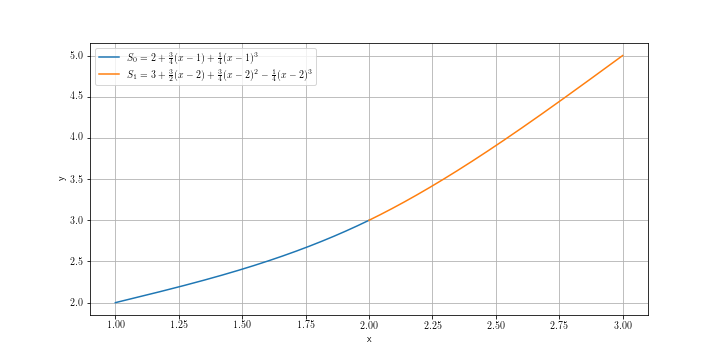
\includegraphics[width=14cm]{Images/ContohCubicSpline}
		\caption{Grafik dari Persamaan \eqref{SPContoh}}
	\end{figure}
	
\end{contoh}


